\documentclass[12pt]{beamer}
\usepackage{beamerthemeHannover, graphicx, clrscode, amsmath, amssymb, multicol}
\usepackage{verbatim}
\setbeamercolor{sidebar}{use=structure,bg=gray!20!red!60!white}
\title{PL/Parrot \\ \small{ Embedding the Parrot Virtual Machine in PostgreSQL } }
\author[Leto+Fetter]{Jonathan "Duke" Leto and David Fetter}
\date{}

\begin{document}

\frame{
    \titlepage
    \begin{center}
    %    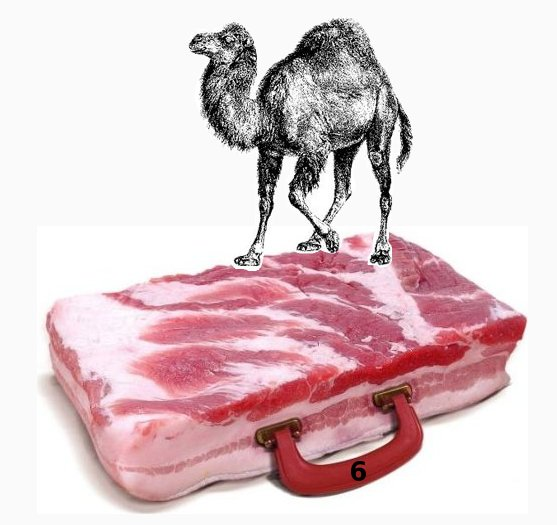
\includegraphics[width=4.57cm, height=4.25cm]{perl6bacon}
    \end{center}
}

\section{What is Parrot Virtual Machine?}
\frame{
    \frametitle{Parrot Virtual Machine}
    \begin{center}
        \begin{itemize}
            \item Process (Application) Virtual Machine
            \item Register-based
            \item Continuation Passing Style
            \item Design Goals
            \begin{itemize}
                \item Pluggable
                \item Interoperable
                \item Dynamic
            \end{itemize}
        \end{itemize}
    \end{center}
}

\section{Why Embed Parrot VM in PostgreSQL?}
\frame{
    \frametitle{Why Embed?}
    \begin{center}
        \begin{itemize}
            \item PL's are (very) hard to write and maintain
            \item Framework for DSL's
            \item Platform independent, fast, stored procedures
            \item Allow various PL's to communicate
            \item Freeze/thaw subtransaction-level states
        \end{itemize}
    \end{center}
}

\section{History of PL/Parrot}
\frame{
    \frametitle{History}
}

\section{Current Features}
\frame{
    \frametitle{Features}
    \begin{itemize}
        \item PL/PIR(U)
        \item Pass and return basic datatypes
        \item Basic security model (Don't do that)
    \end{itemize}
}

\section{Current Bugs/Unimplemented Features}
\frame{
    \frametitle{Bugs}
    \begin{itemize}
        \item Documentation
        \item SPI
        \item Triggers
        \item Parrot Bugs
        \begin{itemize}
            \item IMCC Syntax Errors
            \item Loading libraries from Embed API
        \end{itemize}
    \end{itemize}
}

\section{Example Code}
\frame{
    \frametitle{Code}
    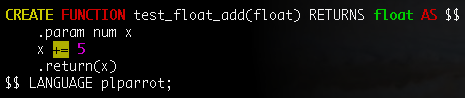
\includegraphics[width=9.5cm, height=3.6cm]{plparrot_example_code}
}


\section{Future Goals}
\frame{
    \frametitle{Future Goals}
    \begin{itemize}
        \item PL/Rakudo - Perl 6 in your database!
        \item PL/Pynie - Python in your Parrot in your database!
        \item Tools to help create a new DSL a.ka. PL on PL/Parrot
    \end{itemize}
}

\section{How to Get Involved}
\frame{
    \frametitle{Get involved}
    \begin{itemize}
        \item GitHub Issues:
        \item Try PL/Parrot on your system and submit detailed bug reports
        \item Fork on github and hack on stuff!
    \end{itemize}
}

\frame{
    \frametitle{ Thanks }
    \begin{itemize}
        \item PL/Parrot team: Joshua Tolley, David E. Wheeler, Daniel Arbelo Arrocha + others
        \item Everyone working on Parrot VM and PostgreSQL
    \end{itemize}
}

\frame{
    \frametitle{ Resources }
    \begin{center}
        \begin{itemize}
           \item http://parrot.org
           \item @parrotvm / !parrot on twitter/identi.ca
           \item \#plparrot on freenode
        \end{itemize}
    \end{center}
}
\end{document}
